\chapter{Taking measurements}
This chapter is going to deal with finding an answer to the question asked in section \ref{subsec:dev-skill-measurement}: how to measure developer skill requirements from job advertisements.
At first, the most frequent commonality between job openings (\ie position description, work location) is determined. Then, the amount of information that can be acquired about developers without their presence is researched. From the common subset, a way to determine developer fit for job openings is derived.

\section{Job advertisement aspects}
We manually analyzed 20 job offers from the Github Jobs site\footnote{\url{https://jobs.github.com} | checked Mai 1, 2015}, which hosts about 300 job offerings, each one valid for 30 days. It became clear that most job offers consisted out of three parts:

\begin{itemize}
  \item A description of the position environment
  \item A detailed description of technical skill requirements
  \item A "wishlist" about the employee character traits
\end{itemize}

Most startup job openings put the emphasis on candidate personality and willingness to learn, as tasks and roles are not yet clearly defined at this stage of company life.\marginpar{Startups define their openings via mindsets and less via requirements. There is often a "can-do, can-learn" attitude.} Phrases like \textit{"An incredibly hard worker, even when it's not so fun"} are quite common and describe a required mindset. For this reason mainly advertisements from larger, established  ompanies were taken into account, because they demand more specifically defined roles.

Inside this subset of openings, for example GitHub and Apple had very specific, measureable technical requirements:
\newline

Apple wants candidates for a data engineer position to
\begin{itemize}
    \item have 3+ years experience with SQL
    \item have 3+ years experience with NoSQL
    \item know Hadoop
\end{itemize}

GitHub wants candidates to have experience with:
\begin{itemize}
    \item web application backend, 3+ years
    \item SQL
    \item Ruby, JavaScript, ElasticSearch optionally
    \item AWS or similar computing solutions optionally
\end{itemize}

Optional qualifications were always mentioned in conjunction with the word "bonus". Presumably, candidates who can supply bonus points are more likely to get hired. While proficiency in a certain programming language is very well verifiable, soft factors like character traits or personal environment preferences are not. For this reason, we are focusing ourselves on analyzing programming skills via written source code, a technique that is described in detail in the next section.

\section{Determining developer skill}
Generally speaking, mastery of something is called a \textit{skill}. Thus, a developer can call mastery of a technology a skill. Measureable is only the code that the developer produces, which is why this code will form the basis for determining individual developer skillsets. This has the advantage that the analysis can take historical data from the code repository into account and be executed without the developers presence. It is neccessary to do so because skills evolve over time, and many job advertisements specifically require a minimum time of acquaintance with a programming language.

\section{Data source}
GitHub is a popular open source community which enjoys high popularity
and hosts the source code repositories of a lot of projects with great influence. These include, but are of course not limited to, Linux, git, docker, elasticsearch, flask and mongo\cite{rpfd:2014}. More importantly, technical recruiters value profiles in such communities greatly from applicants\cite{md:2013}, so there is an added incentive to this datasource. As repositories often contain the combined works of multiple team members, it is important that only individual contributions are measured.

On GitHub there is a distinction between public and private repositories. Public repositories can be read by anyone, while private repositories contain source code disclosed only to a very limited number of people. Analyzing closed source repositories is not an option, as there are lots of privacy and security concerns. That is why the analysis will be restricted to open source repositories that the respective candidate has contributed to. Proposals on how to include mined data from these repositories can be found in chapter \ref{sec:future-work}.
\newline


Judging from the results of a small survey at the german Hasso-Plattner-Institute, chances are that most passionate software developers own a GitHub account.\footnote{The survey reached 608 people.}
\marginpar{96 out of 97 participants at HPI use GitHub.
608 HPI students and alumni were asked in this survey.}
As such, GitHub provides a very good basis for data analysis. It offers two types of data that are of importance to us: users and repositories.
\newline

A user provides the following relevant information:
\begin{itemize}
  \item A Name
  \item The number of followers and followings
  \item A location
  \item Availability for hire
  \item E-Mail addresses which were used for committing
\end{itemize}
\vspace{1em}

\noindent A repository contains the development history of a project, which is subdivided into steps, called \textit{commits}. Each commit contains marks changes made to the code. In the following, we will be dealing with commits, which carry the following attributes relevant for us (also depicted in Figure \ref{fig:commit}):

\begin{itemize}
    \item A \textit{date} when the commit was made
    \item An \textit{email} of whom made the commit
    \item A \textit{patch} of the changes made to the code
    \item A SHA1 sum making the commit uniquely identifiable
\end{itemize}

\begin{figure}
    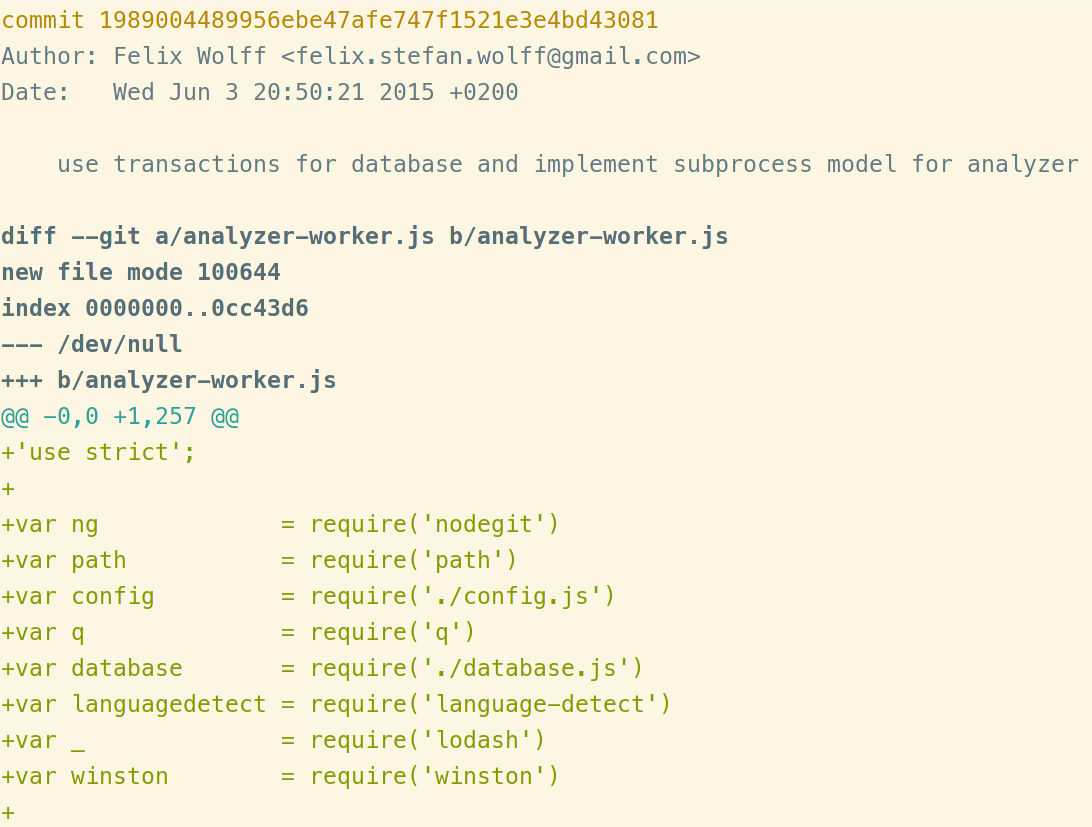
\includegraphics[width=30em]{gfx/commit.png}
    \caption{A sample commit displaying all of the relevant data: date, author with e-mail, diff}
    \label{fig:commit}
\end{figure}

\section{Existing software sizing methods}
Estimating software development effort came up as early as 1981, when Barry W. Boehm invented the \textit{Constructive Cost Model} (COCOMO)\footnote{\url{http://en.wikipedia.org/wiki/COCOMO} | checked June 10, 2015}.
It is a simple measure for estimating code cost based on two main factors: developer count and development time.
\newline

It assumes that more developers will take \textit{less} time to produce the same amount of code, measured in SLOCS\footnote{SLOCS is an abbreviation for \textit{source lines of code}}. This leads to the assumption that more developers produce more code. The project itself does not grow, and thus more developers will finish it faster - a dangerously wrong assumption of historical importance\cite{fb:1975}.
\newline

Research on other measurement methods clearly shows that measuring function points\footnote{\url{http://bit.ly/1C1yys5} | checked June 10, 2015}\footnote{\url{http://bit.ly/1CEmDLy} | checked June 10, 2015} is state-of-the-art for measuring software size and complexity\cite{linkedin:functionpointstandard}. A function point is the unit of measurement that expresses the amount of business functionality a system provides to a user. This is a wholistic measure, meaning that it analyzes the code as-is and does not take into account individual contributions.

Clearly, measuring function points brings comparably better results than counting SLOCs as it is programming language-agnostic and measures the value of user-relevant program features, which makes it more business-relevant. As a side note, counting SLOCs remains present in many companies as processes have been formed around it. Some companies even resorted to paying bonuses for higher line counts\cite{am:2009}.
\newline

Measuring wholistic development effort that has gone into a project as a whole\footnote{\url{http://www.locmetrics.com/alternatives.html} | checked June 10, 2015} is not the approach we need, because it does not take historical data from version control systems into account and makes no distinction between individual contributions.

\section{A custom metric}
This section deals with constructing a metric for answering the research question from \ref{subsec:dev-skill-measurement}. We decided to construct a new metric for this. Most large-scale projects make use of more than one programming language or technology\footnote{see \eg the \href{http://projects.apache.org/indexes/language.html}{Apache Software Foundation Programming Language Index}}, which is why language-sensitivity needs to be part of our metric. The analyzed job offers ask for a minimum experience level with a certain technology, which is why it should consider the experience level as well.

\subsection{A naive approach}
The data available to us consisted strictly out of commits and code statistics. Two assumptions were as follows:

\begin{itemize}
 \item The more experienced a developer, the more code he has seen and written. This experience maps to a timespan worth of work with this technology.
 \item Every human being is different, and as such, developers might have different learning paces. To attribute these, it makes sense to have experience as an abstract measure. This allows the metric to rank fast learners and slow learners on the same level, where the slow learner simply had more time.
\end{itemize}

Unfortunately, the only measurement we were able to make is the number of lines written. As outlined in the previous chapter, measuring SLOC is widely regarded as a bad practice beacause it simply cannot be determined whether the writing of a single line has taken ten seconds or five hours. And again, the kind of language used plays a huge role. On the one hand, a single line of ASM does take less time to write than a single line in JavaScript and will have very little effect on data in main memory. On the other hand, the line in ASM is much harder to write, because the whole memory structure needs to be understood. The answer which line is worth more in this case is very hard to answer. It is dependant on lots of factors - some of which are measurable and some of which are soft. Unfortunately, there is not a lot of research available on the topic of line-based measurements. Many opinionated articles exist\footnote{\url{http://bit.ly/1BRku4a} | checked June 29, 2015}\footnote{\url{http://bit.ly/1BRkAso} | checked June 29, 2015}\footnote{\url{http://bit.ly/1GVzugg} | checked June 29, 2015}, which was evidence enough for us that this approach should be avoided.

\subsection{Technical fit}\label{sec:technicalfit}
From the data that each commit sports it is possible to say when a developer used a programming language for the first time in a project. By aggregating the data over several repositories, it is possible to say when he has used it for the first time in general on GitHub. This resolution of experience is based on timestamps and not on SLOC, which has the disadvantage of being not accessible for fast learners but relieves us of the neccessity to define a mapping of SLOC to a timespan. By using the first and last dates for commits that were made with a certain language, the timespan of experience with this language can easily be calculated, like in formula \ref{eq:timespan}.

\begin{align}
\begin{split}\label{eq:timespan}
timespan(language) ={}& date(lastcommit(language)) - \\
                      & date(firstcommit(language))
\end{split}
\end{align}

This simple calculation alone bears the fallacy that people who use a programming language rarely but every few years get attributed lots of experience. This is solved by the introduction of a \textit{productivity parameter}, which is based off the number of commits one makes per day - as formula \ref{eq:productivity} shows.

\begin{equation}
productivity(language) = \frac{numberofcommits(language)}{timespan(language)}
\label{eq:productivity}
\end{equation}

There is a downside to this, however. It rewards people who commit large files of source code they have not written. A good example might be a commit that contains the \textit{node\_modules} library folder from a Node.js project. In a single commit, this developer will have been attributed thousands of lines of JavaScript.

Small commits are preferred \cite{so:commitsize} over very large commits as they provide a better level of granularity for reverting\footnote{git revert} or cherry-picking\footnote{git cherry-pick}. For this reason, they have become more or less of a standard in free  open source software projects, with 50\% percent of all commits being reasonably small\cite{rsk:2014}. With this in mind, it makes sense to introduce another factor into the metric that gives credit to developers who make small commits, allowing for better teamplay:

\begin{equation}
averageCommitSize(language) = \frac{\sum_{c \in commits(language)} lines(c)}{count(commits)}
\label {eq:avgcommitsize}
\end{equation}

Ranking by the three values, the developers best suited for a position \textit{from the technical perspective} are the ones who have the \textit{greatest timespans}, the \textit{highest productivity}, but the \textit{lowest averageCommitSize}. This metric tries only to capture experience with programming languages, and not experience with technologies.

\subsection{Cultural fit}
Technical competencies aside, nobody wants to work with someone who does not "fit in". A technical fit does not guarantee such a cultural fit. GitHub provides precious little data for gaining insight into the personality of a user.
\newline

A small indicator about the poularity of someone might be the way his profile is valued. On GitHub, users can follow each other and be notified of the actions of their followings. The value of these counters might be a hint of importance and social acceptance.
\newline

GitHub used to provide users with the possibility to write about themselves. Their API still provides a way to read this short biography\footnote{\url{https://developer.github.com/v3/users/} | checked June 29, 2015}, but that is unfortunately a remnant of its removal. This data will be removed in a future version, which was confirmed upon request (see figure \ref{fig:gapitweet}). Some ideas to gain insight into candidate personality are outlined in section \ref{sec:future-work}.

\begin{figure}
  \centering
  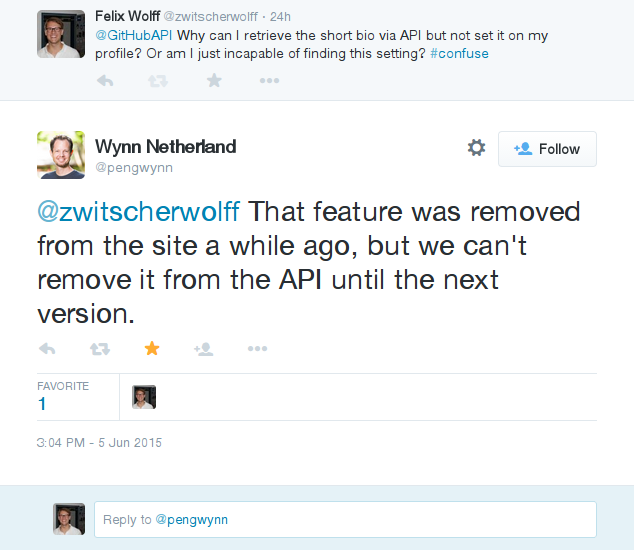
\includegraphics[width=25em]{gfx/githubapi_tweet.png}
  \caption{The tweet that confirmed that the \textit{bio} field is scheduled for removal}
  \label{fig:gapitweet}
\end{figure}

\section{Downsides}\label{sec:threatstovalidity}
For the metric to deliver meaningful results, the base data
needs to be sufficiently large and all e-mail addresses that were used for
making commits need to be registered with the GitHub profile.

Someone who used a open-source component at work, made a small bugfix,
and contributed it back into the project, but left his profile untouched
since then, will not have a very good standing because the data
for attaing one is simply missing. He may even be a very good developer
but any work not published to GitHub will not be considered.